After looking at feature trends and fingerprintability of major
browsers, one interesting question to attempt to answer is this: If
browser fingerprinting is becoming easier over time because Firefox
and Chrome are, in general, becoming more ``bloated'' with features,
does this mean that these browsers are also becoming less secure over
time?  After all, the common folk wisdom is that if a software is more
bloated, it offers more vulnerabilities and a larger attack surface to
launch attacks against (e.g.,~\cite{Bloating}). In this section, we
attempt to answer if there is a direct link between the number of
features a specific browser offers, and the number of vulnerabilities
that have been reported for that browser version.

To answer this question, we extracted the CVE reports for Chrome and
Firefox from 2016 to 2020 as discussed in the methodology section. We
parsed these reports automatically, and generated CVEs that are
related to Google Chrome and Mozilla Firefox for the versions we were
interested in. For Chrome, most CVEs were affecting Google Chrome
49.0.2623 which had 919 reported CVEs. In contrast, Chrome
81.0.4044.129 had the least number of CVEs -- hence, making it the
most secure Google Chrome version. In contrast, for Firefox, 589 CVEs
were reported for Firefox 45 which made it the most vulnerable Firefox
browser in our study. Compared to Firefox 45, Firefox 75 was the most
secure Firefox version in our study with only 11 CVEs. Detailed
information about the number of CVEs reported per browser version is
available in Figures \ref{fig:firefox-vuln} and \ref{fig:chrome-vuln}.

\begin{figure}[ht]
    \centering
    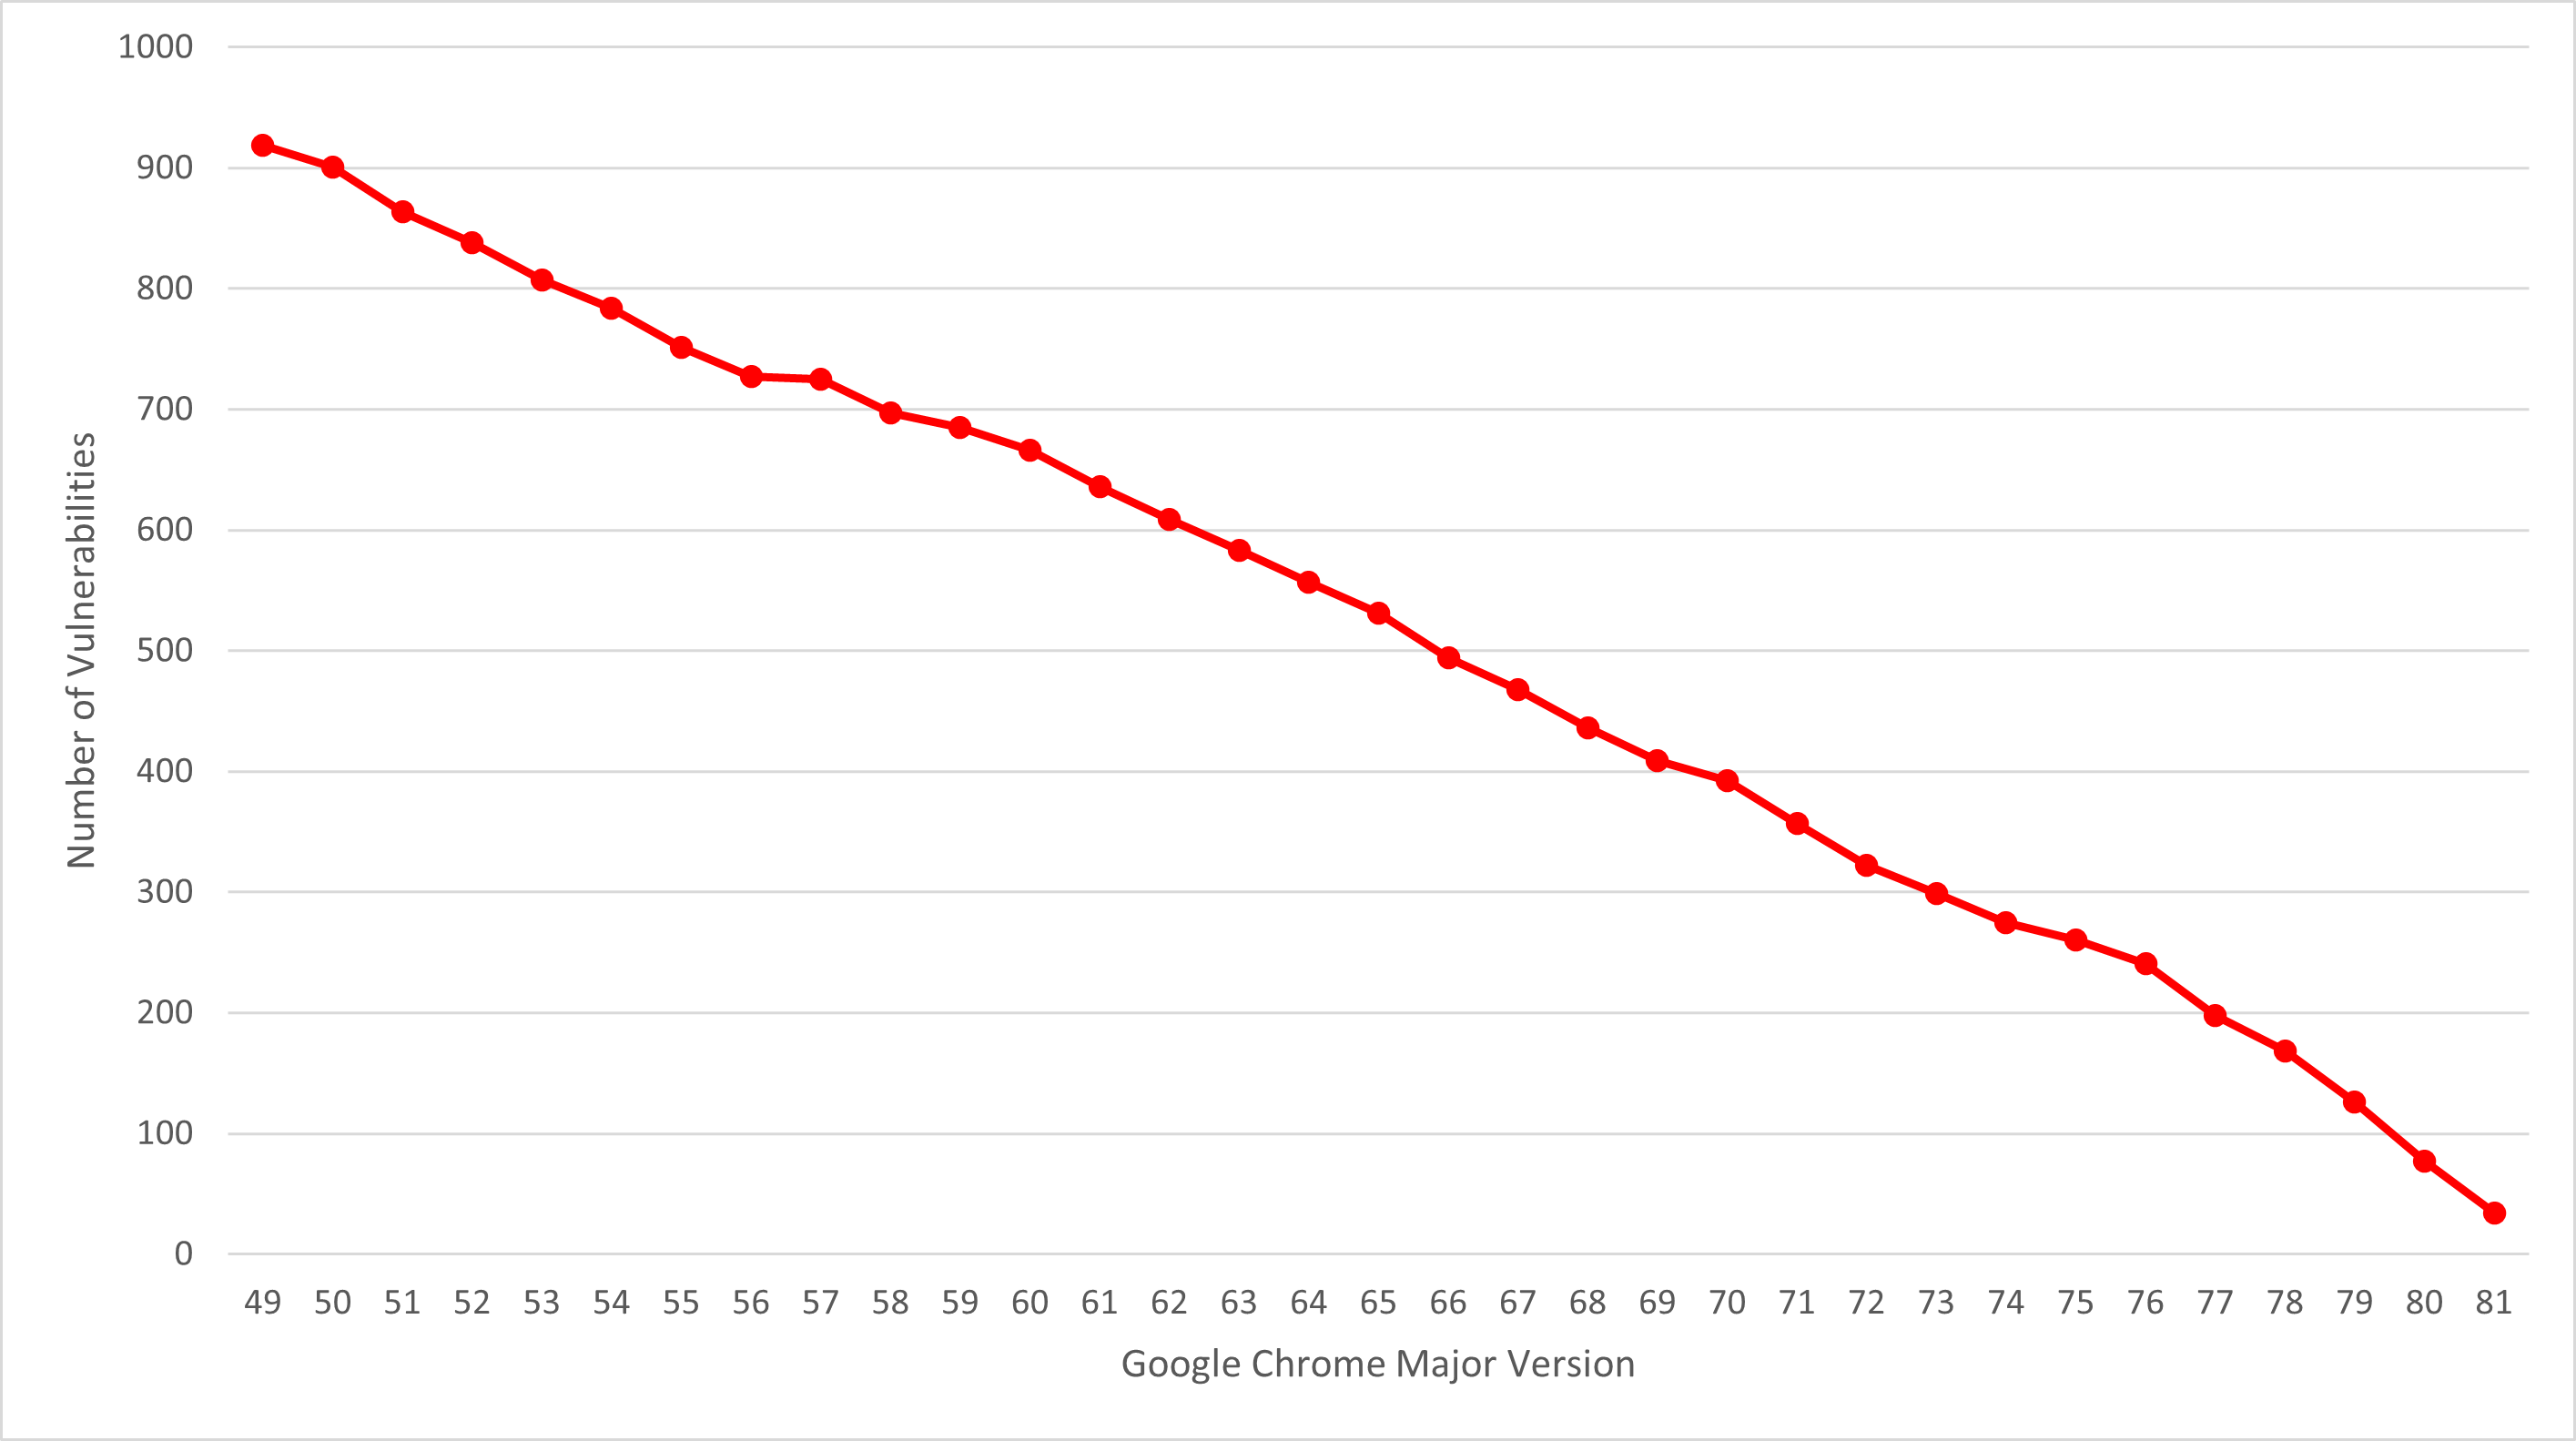
\includegraphics[width=\columnwidth]{figures/Chrome-Vulnerabilities.png}
    \caption{Google Chrome vulnerabilities per version.}
    \label{fig:chrome-vuln}
\end{figure}

\begin{figure}[ht]
    \centering
    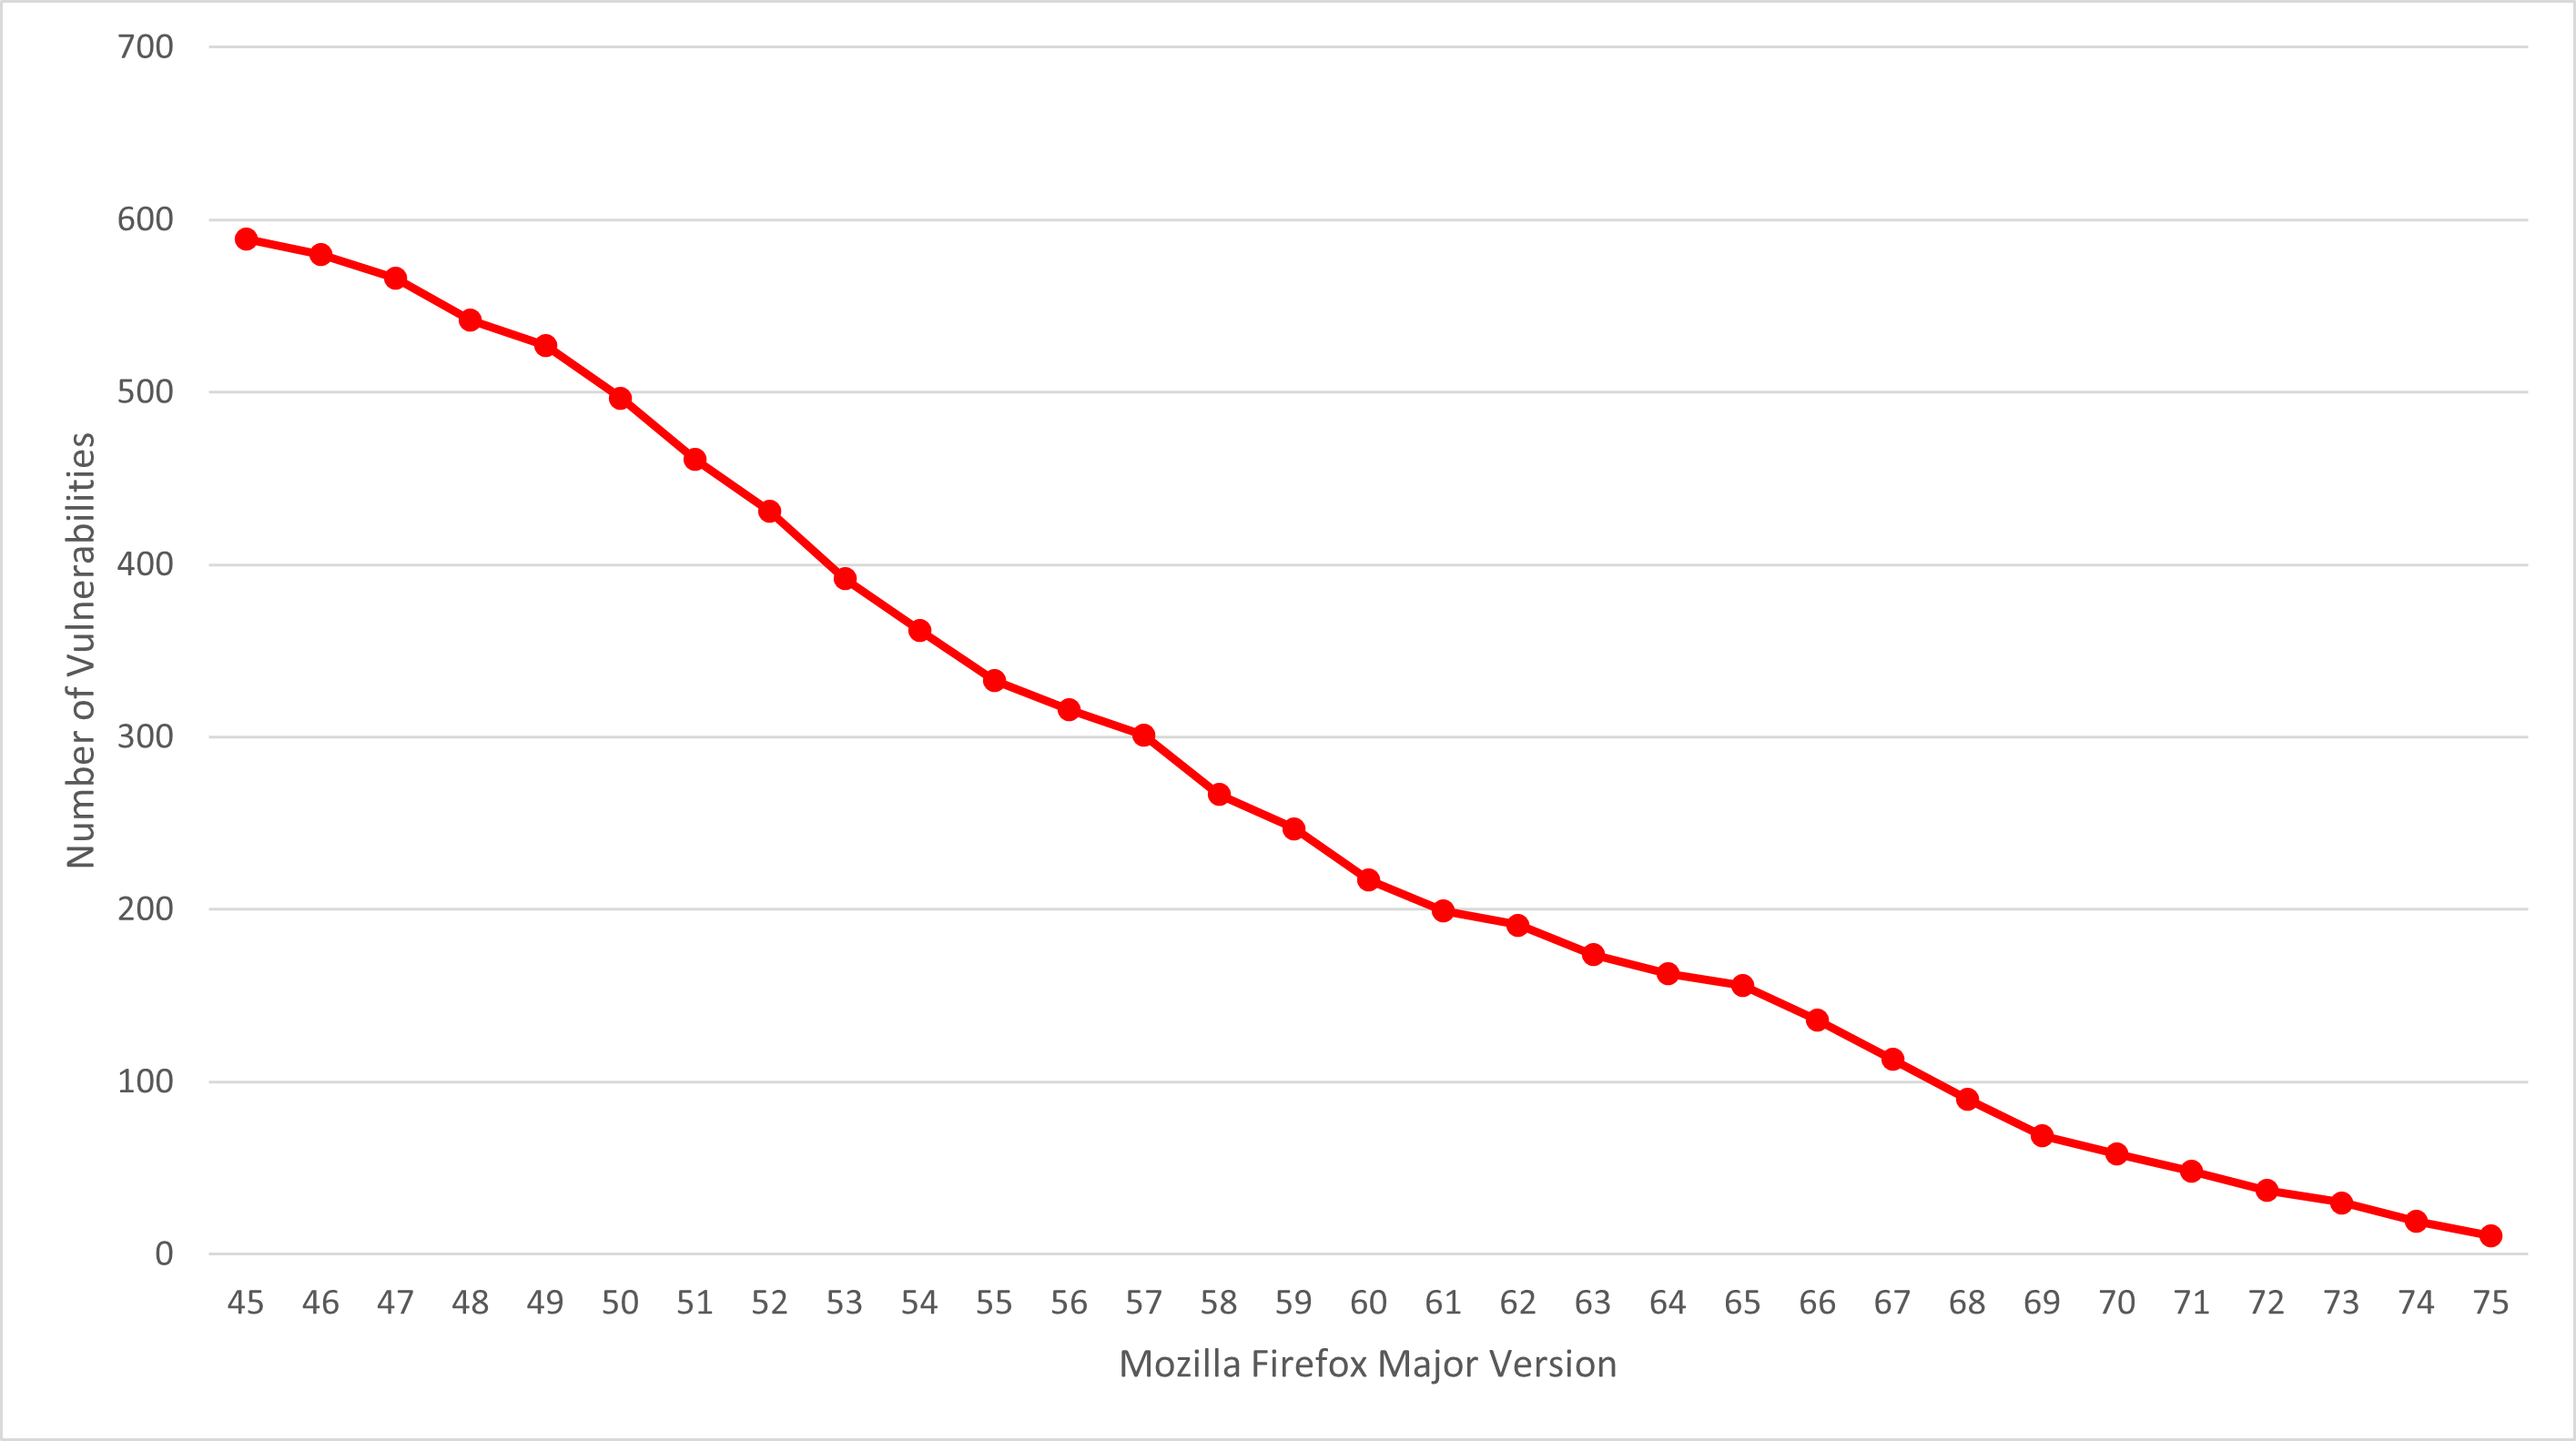
\includegraphics[width=\columnwidth]{figures/Firefox-Vulnerabilities.png}
    \caption{Mozilla Firefox vulnerabilities per version.}
    \label{fig:firefox-vuln}
  \end{figure}


  If we compare CVE date per browser version with the feature trends
  we reported in Figure \ref{fig:featuretrends}, it is evident that
  the increase in the number of reported vulnerabilities does not
  correlate with the increase in the number of supported browser
  features. At first, this might seem counter-intuitive. However, it is
  clear that browser vendors are investing heavily into making their
  browser codebase more robust and secure
  (e.g.,~\cite{FirefoxCrashes,ChromeSecure}). Hence, while the general
  intuition that code ``bloating'' leads to more security problems may
  be correct, at least in the case of browsers, this assumption does
  not seem to hold true.
